\section{逐轮代理模型}
\label{sec:opt-ns-surrogates}

光滑化在开始时一次性地把原目标换成另一个函数，此后只求解替代函数。另一种思路是保留原目标不变，在每一轮围绕当前点重新构造一个容易求解的模型，用模型的最小点作为下一个候选。邻近梯度法已经是这样做的：它每轮使用的二次上界就是一个模型。本节把这一思路推广到两类模型。第一类是处处位于原目标上方、并在当前点接触的上界模型，它直接保证原目标下降，即MM方法；第二类是由已查询的支撑直线拼成的下界模型，它只能预测下降，候选点要查询原目标后才决定是否接受，即束方法。两类模型承担的作用不同，接受规则和保证也不同。

\subsection{MM的构造与更新}
\label{sec:opt-ns-mm}

回到邻近梯度法。式~\eqref{eq:opt-ns-descent-lemma}说明，$0<\eta\leq1/L$时模型$m_{\bm x}(\bm y)$处处不低于$F(\bm y)$，并且$m_{\bm x}(\bm x)=F(\bm x)$。正是这两条性质，加上新点使模型不高于当前值，保证了原目标下降。把这三条要求单独提出来，就不必限于二次上界。

\begin{definition}[主化代理与MM更新]
\label{def:opt-ns-mm}
设$F:\mathbb R^d\to\mathbb R\cup\{+\infty\}$，$\bm x^{(t)}\in\operatorname{dom}F$。函数$Q(\cdot\mid\bm x^{(t)})$若满足
\[
 Q(\bm x\mid\bm x^{(t)})\geq F(\bm x)\ \ \text{对所有}\ \bm x,\qquad Q(\bm x^{(t)}\mid\bm x^{(t)})=F(\bm x^{(t)}),
\]
就称为$F$在$\bm x^{(t)}$处的主化代理（majorizer）。选取满足$Q(\bm x^{(t+1)}\mid\bm x^{(t)})\leq Q(\bm x^{(t)}\mid\bm x^{(t)})$的新点，通常取代理的最小点，这样的迭代称为\term{主化--最小化方法}（majorization--minimization，MM）。
\end{definition}

三项要求依次是全域上界、当前点接触和代理改善。它们连成一条不等式链：
\begin{equation}
 F(\bm x^{(t+1)})\leq Q(\bm x^{(t+1)}\mid\bm x^{(t)})\leq Q(\bm x^{(t)}\mid\bm x^{(t)})=F(\bm x^{(t)}),
 \label{eq:opt-ns-mm-chain}
\end{equation}
第一步用上界，第二步用代理改善，第三步用接触。MM保证原目标逐轮不增，而且不需要原目标可微或凸，只需要能构造合格的代理。

\paragraph{为什么切线不行}
图~\ref{fig:opt-ns-mm-surrogates}左图比较$F(x)=x^2/2$在$x=1$处的两条曲线。主化代理$Q(x\mid1)=(x-1/2)^2+1/4$与$F$同值同斜率，并且$Q-F=(x-1)^2/2\geq0$，所以处处在上方；它的最小点$x=1/2$处$F(1/2)=1/8<1/2$，原目标确实下降。同一点的切线$x-1/2$也与$F$同值同斜率，但凸函数的切线在图像下方，不等式链的第一步反了；而且切线没有最小点，沿它下降会走到无穷远。可见“当前点同值同斜率”远不足以构成代理，关键在于全域的上方关系。

\begin{figure}[!htbp]
  \centering
  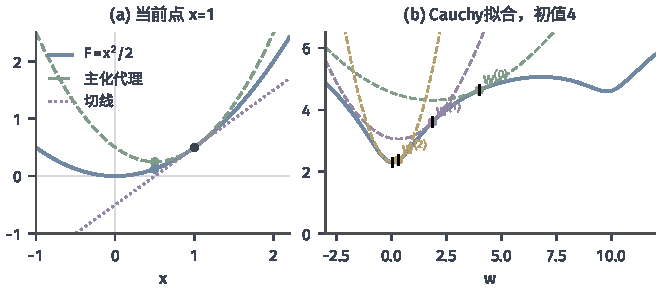
\includegraphics[width=112mm]{figures/03-optimization-evolution-and-signals/01-optimization/matplotlib/c4-mm-surrogates/figure.pdf}
  \caption{主化代理逐轮接触原目标。(a) 蓝线$F(x)=x^2/2$，绿色虚线是$x=1$处的主化代理$(x-1/2)^2+1/4$，紫色点线是同一点的切线$x-1/2$；代理在上方、切线在下方。代理的最小点$1/2$处，原目标从$1/2$降到$1/8$。(b) 蓝线是例~\ref{ex:opt-ns-cauchy-mm}的Cauchy拟合目标，三条虚线是从$w^{(0)}=4$开始前三轮的代理，每条都在当前点（圆点）接触目标、在别处位于上方，其最小点就是下一轮的当前点。}
  \label{fig:opt-ns-mm-surrogates}
\end{figure}

\paragraph{不精确求解代理}
代理子问题往往也要迭代求解，得到的只是近似最小点。记$Q^{\star,(t)}=\min_{\bm x}Q(\bm x\mid\bm x^{(t)})$，以及代理能提供的最大改善量$\Delta^{(t)}=Q(\bm x^{(t)}\mid\bm x^{(t)})-Q^{\star,(t)}\geq0$。若返回点满足$Q(\bm x^{(t+1)}\mid\bm x^{(t)})\leq Q^{\star,(t)}+\epsilon^{(t)}$，则由上界和接触，
\[
 F(\bm x^{(t+1)})\leq Q^{\star,(t)}+\epsilon^{(t)}=F(\bm x^{(t)})-\Delta^{(t)}+\epsilon^{(t)}.
\]
只有子问题误差$\epsilon^{(t)}$不超过可用改善量$\Delta^{(t)}$，本轮才保证不升。在左图的例子中，$Q^{\star}=1/4$，$\Delta=1/2-1/4=1/4$。若返回$x=3/4$，代理值$5/16$，误差$1/16\leq1/4$，原目标$F(3/4)=9/32<1/2$；若返回$x=5/4$，代理值$13/16$，误差$9/16>1/4$，原目标$F(5/4)=25/32$反而高于$1/2$。实现时最简单的检查是直接比较代理值：只要$Q(\bm x^{(t+1)}\mid\bm x^{(t)})\leq Q(\bm x^{(t)}\mid\bm x^{(t)})$，不等式链就成立。

\paragraph{局部代理}
有时上界只在当前点附近的区域$D^{(t)}$内成立，例如二次上界所用的曲率常数只在一个球内有效。这时不等式链的第一步只对$D^{(t)}$中的点成立，候选点必须限制在$D^{(t)}$内，代理子问题相应地带上这个约束。若不加限制地最小化代理，新点可能落在区域外，链就断了；局部有效的上界不能被无声地当作全局上界使用。

\paragraph{由凹性构造代理}
构造代理最常用的工具是凹函数在切线下方。设$\rho:[0,\infty)\to\mathbb R$可微、非减且凹，则$\rho(s)\leq\rho(s_0)+\rho'(s_0)(s-s_0)$对所有$s,s_0\geq0$成立。若目标形如$F(\bm x)=\frac12\sum_i\rho\bigl(r_i(\bm x)^2\bigr)$，其中$r_i$是残差，把每一项在当前残差平方$s_i^{(t)}=r_i(\bm x^{(t)})^2$处线性化，就得到
\begin{equation}
 Q(\bm x\mid\bm x^{(t)})=F(\bm x^{(t)})+\frac12\sum_ia_i^{(t)}\bigl(r_i(\bm x)^2-r_i(\bm x^{(t)})^2\bigr),\qquad a_i^{(t)}=\rho'(s_i^{(t)})\geq0 .
 \label{eq:opt-ns-irls-surrogate}
\end{equation}
它满足上界与接触两项要求，并且是残差的加权平方和：残差线性时，最小化代理就是一个加权最小二乘问题。每轮“由当前残差算权重、解加权最小二乘、更新残差”的方法称为\term{迭代重加权最小二乘}（iteratively reweighted least squares，IRLS）。拟合中的残差设计、权重退化与线性子问题的求解在第~\ref{chap:opt-function-fitting}章展开，这里只用一个标量例说明代理的构造。

\begin{example}[Cauchy损失的MM迭代]
\label{ex:opt-ns-cauchy-mm}
用一个常数$w$拟合数据$y=(0,0,10)$，目标为$F(w)=\frac12\sum_{i=1}^3\log\bigl(1+(w-y_i)^2\bigr)$，即$\rho(s)=\log(1+s)$，它凹且非减，$\rho'(s)=1/(1+s)$。由式~\eqref{eq:opt-ns-irls-surrogate}，代理的最小点是加权平均$w^{(t+1)}=\sum_ia_i^{(t)}y_i/\sum_ia_i^{(t)}$，权重$a_i^{(t)}=1/\bigl(1+(w^{(t)}-y_i)^2\bigr)$。

从$w^{(0)}=4$出发，权重为$(1/17,1/17,1/37)$，加权平均为$w^{(1)}=\frac{10/37}{2/17+1/37}\approx1.868$；下一轮权重约为$(0.223,0.223,0.015)$，得$w^{(2)}\approx0.324$；再下一轮得$w^{(3)}\approx0.058$。离群点$10$的权重随着它的残差增大而迅速变小，迭代趋向局部最小点$w\approx0.050$。从$w^{(0)}=0$出发，第一步权重为$(1,1,1/101)$，得$w^{(1)}=10/203\approx0.049$。图~\ref{fig:opt-ns-mm-surrogates}右图画出从$4$出发的前三个代理，每个都在当前点接触目标、在别处位于上方。

这个目标不是凸的，它在$w\approx9.789$处还有一个目标值更大的局部最小点（约$4.595$，而前者约$2.305$）。从$w^{(0)}=8$出发，MM迭代单调地收敛到$9.789$附近。不等式链只保证目标值不增，不保证到达全局最小点。
\end{example}

MM的适用范围不限于非光滑目标；光滑目标同样可以用二次上界或凹线性化构造代理。把它放在本章，是因为它与下面的束方法、上一节的光滑化一起，回答同一个问题：当原目标不便直接处理时，用什么样的辅助模型推进迭代。

\subsection{束方法}
\label{sec:opt-ns-bundle}

次梯度法每轮只用当前这一条支撑直线，用过就丢。对凸目标，每条查询到的支撑直线在全空间都是有效的下界，丢掉它们很浪费。\term{束方法}（bundle method）把查询过的支撑直线都保存下来，拼成原目标的一个分段线性下界模型，再加一个距离项防止候选点跑得太远。

\paragraph{割平面模型与稳定中心}
设$F:\mathbb R^d\to\mathbb R$是有限值凸函数，查询程序对每个点$\bm y$返回$F(\bm y)$和一条$\bm g\in\partial F(\bm y)$。设已经查询了点$\bm y_0,\dots,\bm y_k$，对应次梯度$\bm g_0,\dots,\bm g_k$。由支撑不等式，每条直线都在$F$下方，它们的最大值
\[
 m_k(\bm x)=\max_{0\leq j\leq k}\bigl\{F(\bm y_j)+\langle\bm g_j,\bm x-\bm y_j\rangle\bigr\}\leq F(\bm x)
\]
称为割平面模型，保存的这些直线合称为“束”。模型在每个查询点处与$F$相等，在其他地方是下界，越往查询点之外走，模型低估得越厉害。

只最小化$m_k$是危险的：它可能没有下界，例如只有一条支撑直线时；即使有最小点，也可能远离已知信息可靠的区域。因此束方法另外维护一个\term{稳定中心}（stability center）$\hat{\bm x}_k$，它是目前目标值最好的已接受点，并求解
\begin{equation}
 \bm y_{k+1}=\argmin_{\bm x}\Bigl\{m_k(\bm x)+\frac1{2\tau}\lVert\bm x-\hat{\bm x}_k\rVert_2^2\Bigr\}=\operatorname{prox}_{\tau m_k}(\hat{\bm x}_k),
 \label{eq:opt-ns-bundle-candidate}
\end{equation}
其中$\tau>0$。这是第~\ref{sec:opt-ns-prox}节的邻近子问题，只是把原目标换成了它的割平面模型：由定理~\ref{thm:opt-ns-prox-characterization}，解存在唯一。引入辅助变量$q$表示模型值，它可以写成二次规划：在约束$q\geq F(\bm y_j)+\langle\bm g_j,\bm x-\bm y_j\rangle$（$j=0,\dots,k$）下最小化$q+\lVert\bm x-\hat{\bm x}_k\rVert_2^2/(2\tau)$。

\paragraph{预测下降与接受检验}
模型在中心处是精确的（只要中心处的支撑直线在束中），所以$m_k(\hat{\bm x}_k)=F(\hat{\bm x}_k)$。模型预测，从中心移到候选点能使目标降低
\[
 \delta_k=F(\hat{\bm x}_k)-m_k(\bm y_{k+1}).
\]
由于$\bm y_{k+1}$是子问题的最小点，$m_k(\bm y_{k+1})+\lVert\bm y_{k+1}-\hat{\bm x}_k\rVert_2^2/(2\tau)\leq m_k(\hat{\bm x}_k)=F(\hat{\bm x}_k)$，所以$\delta_k\geq0$。但模型是下界，预测往往过于乐观，必须查询$F(\bm y_{k+1})$核验。给定$\beta\in(0,1)$，若实际下降至少是预测的$\beta$倍，
\[
 F(\hat{\bm x}_k)-F(\bm y_{k+1})\geq\beta\,\delta_k ,
\]
就接受候选点为新中心，称为\term{实质步}（serious step）；否则中心不动，称为\term{空步}（null step）。无论哪种情况，都把$\bm y_{k+1}$处的新支撑直线加入束。空步没有移动中心，却在模型低估最严重的地方补了一条割线，使下一次预测更准。

\begin{algorithm}[邻近束方法]
  \label{alg:opt-ns-bundle}
  \begin{algorithmic}[1]
    \Require 有限值凸函数$F$的函数值与次梯度程序；初值$\bm y_0$；参数$\tau>0$，$\beta\in(0,1)$；容差$\varepsilon$
    \Ensure 稳定中心$\hat{\bm x}$及证书$(e,\bm s)$
    \State 查询$F(\bm y_0)$与$\bm g_0$，束$\gets\{(\bm y_0,F(\bm y_0),\bm g_0)\}$，$\hat{\bm x}\gets\bm y_0$
    \For{$k=0,1,2,\dots$}
      \State 由式~\eqref{eq:opt-ns-bundle-candidate}求候选$\bm y_{k+1}$，计算$\delta_k=F(\hat{\bm x})-m_k(\bm y_{k+1})$
      \State $\bm s\gets(\hat{\bm x}-\bm y_{k+1})/\tau$，$e\gets\delta_k-\tau\lVert\bm s\rVert_2^2$
      \If{$\delta_k\leq\varepsilon$}
        \State \Return $\hat{\bm x}$，$(e,\bm s)$
      \EndIf
      \State 查询$F(\bm y_{k+1})$与$\bm g_{k+1}\in\partial F(\bm y_{k+1})$，把这条支撑直线加入束
      \If{$F(\hat{\bm x})-F(\bm y_{k+1})\geq\beta\delta_k$}
        \State $\hat{\bm x}\gets\bm y_{k+1}$ \Comment{实质步}
      \EndIf \Comment{否则为空步，中心不动}
    \EndFor
  \end{algorithmic}
\end{algorithm}

\begin{example}[一维束方法]
\label{ex:opt-ns-bundle-1d}
取$F(x)=|x-1|+x^2/4$，最小点$x^\star=1$，$F^\star=1/4$。查询程序在$x<1$时返回$x/2-1$，在$x\geq1$时返回$x/2+1$。取$\tau=1$、$\beta=1/2$，从$y_0=-2$出发。

第一轮：$F(-2)=4$，$g_0=-2$，模型$m_0(x)=4-2(x+2)=-2x$。子问题$-2x+(x+2)^2/2$的最小点是$y_1=0$，预测下降$\delta_0=4-0=4$；实际$F(0)=1$，下降$3\geq2$，实质步，中心移到$0$。注意$m_0$本身没有下界，正是距离项让子问题有解。

第二轮：加入$0$处的割线$1-x$，模型为$\max\{-2x,1-x\}$。子问题在$x>-1$时为$1-x+x^2/2$，最小点$y_2=1$，模型值$0$，预测下降$1$；实际$F(1)=1/4$，下降$3/4\geq1/2$，实质步，中心移到$1$。

第三轮：加入$1$处的割线$1/4+\tfrac32(x-1)$。在中心$1$附近，模型由$1-x$与这条新割线组成，两者交于$x=0.9$，模型值$0.1$；子问题的最小点就是$y_3=0.9$（模型在此的次微分$[-1,3/2]$加上距离项斜率$-0.1$含零）。预测下降$\delta_2=0.15$，实际$F(0.9)=0.3025$反而比中心高，空步。第四轮加入$0.9$处的割线后，候选点约为$0.9988$，预测下降只有约$0.0018$，实际目标约$0.2506$，仍是空步，但此时预测下降已经很小。图~\ref{fig:opt-ns-bundle}画出第二、三轮的模型。
\end{example}

\begin{figure}[!htbp]
  \centering
  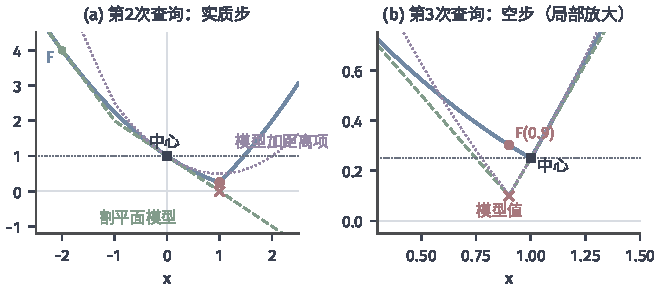
\includegraphics[width=112mm]{figures/03-optimization-evolution-and-signals/01-optimization/matplotlib/c4-bundle-model/figure.pdf}
  \caption{邻近束方法在$F(x)=|x-1|+x^2/4$上的两轮（例~\ref{ex:opt-ns-bundle-1d}，$\tau=1$）。蓝线是$F$，绿色虚线是由已查询点（绿点）的支撑直线拼成的割平面模型，紫色点线是模型加距离项，黑色方块是稳定中心，灰色点线标出中心处的目标值。红叉是候选点处的模型值，红点是候选点处的真实目标值。(a) 中心在$0$，候选点$1$的真实下降达到预测的一半以上，实质步。(b) 局部放大：中心在$1$，模型预测候选点$0.9$处的值为$0.1$，真实值却是$0.3025$，高于中心，空步。}
  \label{fig:opt-ns-bundle}
\end{figure}

\paragraph{可核验的停止标准}
预测下降不仅决定接受与否，还给出最优性证书。由于$\bm y_{k+1}=\operatorname{prox}_{\tau m_k}(\hat{\bm x}_k)$，邻近最优条件给出$\bm s_k=(\hat{\bm x}_k-\bm y_{k+1})/\tau\in\partial m_k(\bm y_{k+1})$。于是对所有$\bm x$，
\[
 F(\bm x)\geq m_k(\bm x)\geq m_k(\bm y_{k+1})+\langle\bm s_k,\bm x-\bm y_{k+1}\rangle
 =F(\hat{\bm x}_k)+\langle\bm s_k,\bm x-\hat{\bm x}_k\rangle-e_k ,
\]
其中$e_k=\delta_k-\tau\lVert\bm s_k\rVert_2^2$；最后一步用了$m_k(\bm y_{k+1})=F(\hat{\bm x}_k)-\delta_k$与$\langle\bm s_k,\hat{\bm x}_k-\bm y_{k+1}\rangle=\tau\lVert\bm s_k\rVert_2^2$。在上式中取$\bm x=\hat{\bm x}_k$，得$e_k\geq0$，因此$\tau\lVert\bm s_k\rVert_2^2\leq\delta_k$且$e_k\leq\delta_k$。上式说明$\bm s_k$是一条带误差$e_k$的近似次梯度；若已知某个最小点满足$\lVert\hat{\bm x}_k-\bm x^\star\rVert_2\leq R$，取$\bm x=\bm x^\star$即得
\[
 F(\hat{\bm x}_k)-F^\star\leq e_k+R\lVert\bm s_k\rVert_2\leq\delta_k+R\sqrt{\delta_k/\tau}.
\]
所以$\delta_k$小就同时控制了线性化误差和近似次梯度的大小。在例~\ref{ex:opt-ns-bundle-1d}第四轮，$\delta\approx0.0018$，$\lVert s\rVert=0.0012$，中心$1$正是最小点。

\paragraph{计算预算}
束方法的迭代次数不等于中心移动的次数。每一轮都要查询一次原目标（无论实质步还是空步）并求解一个二次规划，而二次规划的约束个数随束的增长而增长。报告计算量时要同时计入实质步、空步、原目标查询次数和每次子问题的求解代价；实践中还会定期合并或删去不再活跃的割线来控制束的大小，这需要额外的规则保证模型仍然有效。

\subsection{代理的保证与结果检验}
\label{sec:opt-ns-surrogate-guarantees}

上界模型、下界模型和固定的光滑替代都在用一个辅助函数推进迭代，但它们对原目标说了不同的话。本小节把三者放在同一个原目标下对照。

\paragraph{上模型与下模型不能互换}
MM的上界模型给出的是保证：代理值下降多少，原目标至少下降多少，由不等式链~\eqref{eq:opt-ns-mm-chain}直接得到，无需查询原目标。束方法的下界模型给出的只是预测：模型值下降，原目标可能上升，例~\ref{ex:opt-ns-bundle-1d}第三轮就是如此，所以每个候选点都必须查询原目标并通过接受检验。反过来，下界模型有上界模型没有的东西：它积累的割线给出了$F^\star$的下界和停止证书，而MM只能告诉我们目标值在下降，不能说明离最优还有多远。把下界模型当作上界使用会失去下降保证；把上界模型的最小值当作最优值的下界则是错误的。

光滑化又是第三种情形。它不在每轮重建模型，而是固定一个与原目标处处相差不超过$\nu\log m$的替代函数，然后只求解替代函数；它对原目标的控制完全来自偏差界~\eqref{eq:opt-ns-lse-gap}和误差分解~\eqref{eq:opt-ns-smoothing-split}，原目标在中间某些轮上升是允许的。表~\ref{tab:opt-ns-surrogates}汇总了三者的区别。

\begin{table}[!htbp]
  \centering
  \small
  \begin{tabularx}{\linewidth}{@{}l>{\raggedright\arraybackslash}X>{\raggedright\arraybackslash}X>{\raggedright\arraybackslash}X@{}}
    \toprule
     & MM & 束方法 & 光滑化 \\
    \midrule
    辅助函数 & 当前点处的主化代理，每轮重建 & 割平面下界模型，逐轮加割线 & 固定的光滑替代 \\
    与原目标的关系 & 处处在上方，当前点接触 & 处处在下方，查询点处相等 & 相差不超过$\nu\log m$ \\
    接受规则 & 代理值不增即可，无需查询原目标 & 实际下降不少于预测的$\beta$倍 & 无，按替代目标的方法运行 \\
    逐轮原目标 & 不增 & 中心处不增，候选点可升 & 可升，上升不超过$\nu\log m$ \\
    给出的保证 & 目标值单调；无最优间隙 & 停止证书$e_k+R\lVert\bm s_k\rVert_2$ & 原目标误差$\leq$优化误差$+\nu\log m$ \\
    \bottomrule
  \end{tabularx}
  \caption{三种辅助模型的对照。三者都作用于同一个原目标，但辅助函数与原目标的关系不同，因而接受规则和能报告的保证不同。}
  \label{tab:opt-ns-surrogates}
\end{table}

\paragraph{成本与返回对象}
三种方法的代价落在不同环节。MM的代价在构造代理和求解代理子问题，例如IRLS每轮解一个加权最小二乘；子问题只要求代理值不增，可以不精确求解。束方法的代价在原目标查询与越来越大的二次规划，空步消耗查询却不移动中心。光滑化的代价在梯度方法的迭代次数，它随$1/\nu$增长，改变$\nu$还要重新确定步长。返回时也要分清对象：MM返回最后一个迭代点；束方法返回稳定中心，而不是最后一个候选点，后者可能比中心差；光滑化返回替代问题的近似解，报告时应同时给出它的原目标值。

\paragraph{目标值收敛之后}
MM和束方法的中心都使原目标单调不增。若原目标有下界，单调有界的数列收敛，所以目标值序列收敛；但这只是目标值的收敛。迭代点是否收敛、极限是否为驻点、是否为全局最小点，都需要另外的条件。例~\ref{ex:opt-ns-cauchy-mm}从$8$出发收敛到一个非全局的局部最小点；对MM，证明极限点是驻点通常还要求代理在接触点处与目标的方向导数一致、代理关于当前点连续等条件。凸目标上束方法的收敛分析需要同时处理实质步与空步序列，篇幅较长，本章不展开，只使用上面可逐轮核验的停止证书：它不依赖收敛定理，每一轮都可以直接计算。
